\chapter{L'SGBD RRDtool}\label{cap:rrdtool}

En aquest capítol s'introdueix el sistema de gestió de bases de dades RRDtool, l'únic sistema operatiu conegut actualment que utilitza el model de dades Round Robin (RRD). 
També s'explica com funciona RRDtool des del punt de vista d'un usuari; per a més detall en el capítol següent s'explica el funcionament intern.  


L'estructura d'aquest capítol ofereix incrementalment els conceptes bàsics de RRDtool. 
Primer s'introdueix el motiu de creació de  RRDtool i les solucions que vol aportar.
 
En segon lloc, es descriu el model que utilitza RRDtool, el model RRD, utilitzant vocabulari  habitual en altres bases de dades, el qual potser és més conegut pel lector. Com que RRDtool és una base de dades, no es pot deixar de banda una explicació breu del gestor de bases de dades, en aquest cas no es contemplen  els aspectes més informàtics i només es fa una equivalència entre vocabulari habitual de les bases de dades i implementació a RRDtool. 


Tot seguit, s'explica el que caracteritza a RRDtool: l'estructura Round Robin. A causa d'aquesta estructura es necessita tractar les sèries temporals, el qual s'explica a través de la interpolació i la consolidació de les dades. Per tancar amb l'estructura, s'enumeren els tipus de dades que admet RRDtool.


Finalment, s'explica les operacions que es poden fer amb RDDtool i la sintaxi del llenguatge d'interacció amb la base de dades. Es destaca la curiosa implementació d'operacions per presentar gràficament les dades.




\section{Introducció}

RRDtool (Round Robin Database Tool), \cite{rrdtool}, és un SGBD per enregistrar i visualitzar dades estructurades com a sèries temporals i, actualment, és l'estàndard \emph{de facto} en l'àmbit del programari lliure. L'objectiu principal de RRDtool és tractar sèries temporals, mantenint la coherència i la lògica que requereix el monitoratge de dades de la manera més ràpida i senzilla possible i ocupant el mínim d'espai.

Inicialment, formava part del programa de monitoratge \emph{Multi Router Traffic Grapher}, (MRTG)~\cite{mrtg}, però posteriorment ha esdevingut una part separada amb característiques i funcionament independent, segons explica Oetiker a~\cite{lisa98:oetiker}. Durant aquest període de temps, RRDTool ha anat evolucionant fins a tenir una estructura dissenyada específicament per tractar dades en sèries temporals. Finalment, aquest disseny propi ha estat classificat com un model de dades Round Robin (RRD, \emph{Round Robin Database}). 

El nom Round Robin prové principalment de la manera d'emmagatzemar les sèries temporals. Aquest emmagatzematge consisteix en desar cada valor en un arxiu que té un punter, el qual va recorrent els valors tot apuntant al que s'ha de llegir o escriure en cada moment. 
Això recorda als mètodes que recorren elements d'un grup de manera equitativa i ordenada, començant pel primer i tornant a començar quan s'arriba a l'últim, els quals s'anomenen mètodes \emph{Round Robin}. 
A més a més, a RDDtool els arxius sempre tenen la mateixa mida d'elements; la mida es defineix en crear la base de dades i així s'eviten els problemes de creixement indeterminat que tenen altres bases de dades.

A banda de tenir un emmagatzematge Round Robin, RRDtool té més tècniques específiques per tractar sèries temporals, les quals han de tenir en compte el model Round Robin.

Una d'aquestes tècniques consisteix en conservar un sèrie temporal amb diferents resolucions de temps, a on cadascuna es pot anomenar 'finestra temporal'. Cada finestra conserva la sèrie temporal fins a un límit de temps, de manera que les dades més recents en el temps es desen amb més resolució però la perden a mesura que es tornen velles. 
Així es pot consultar la finestra temporal més adient en cada cas, considerant que cal detall en les finestres amb dades més recents però que es pot relaxar la resolució en les finestres que conserven intervals de temps més grans.

Aquesta solució d'emmagatzematge comporta una pèrdua de dades, ja que la informació perd resolució en el temps. Ara bé, aquesta pèrdua permet obtenir avantatges com per exemple un càlcul més àgil amb les dades, que la mida emmagatzemada no creixi en el temps o que la visualització de gràfics sigui més ràpida.

%A més a més, les RRD classifiquen les dades en diferents tipus i apliquen un tractament diferenciat a cada una.

Cal destacar que la generació àgil de gràfics és un altre dels objectius principals de RRDtool, ja que es considera una part important en les interfícies persona-màquina dels sistemes de monitoratge. El benefici de RRDtool és no haver d'estar pendent del sistema de monitoratge ni del d'emmagatzematge i poder-se centrar en l'anàlisi visual de les dades, obtenint el major tractament i anàlisi automàtic possible per part de RRDtool.

Finalment, la implementació d'aquestes tècniques específiques ha comportat que RRDtool tingui un llenguatge propi per operar amb la base de dades. Així doncs, no implementa els llenguatges estàndards de bases de dades, com pot ser l'\emph{Structured Query Language} (SQL, estàndard ISO/IEC 9075) utilitzat en les bases de dades relacionals. Això és degut a que les operacions a RRDtool només tenen sentit per sèries temporals i per exemple, amb referència als gràfics, hi ha una operació que serveix per representar gràficament.




\section{Comparació amb altres SGBD}

Estructuralment i comparant amb altres bases de dades, tenint com a referència bàsica a Date~\cite{date}, una base de dades RRDtool és una taula que pot tenir més d'un camp però amb el nombre de registres fixos. El primer camp és la clau única i és on es desa la data i hora d'entrada de dades al registre. Els camps poden ser valors d'un mateix recurs o no tenir res a veure però sempre comparteixen el mateix temps de mesura, és a dir que s'han d'inserir tots els camps a la vegada.

Les operacions que permet RRDtool són les d'inserir i consultar dades i augmentar i disminuir els registres. Per la seva pròpia naturalesa no pot eliminar o afegir registres concrets sinó que les operacions d'augmentar i disminuir treballen amb els registres més vells.  Tampoc pot canviar dades de registres existents i les dades s'han d'inserir seqüencialment en el temps.

Així doncs, per poder desar valors a RRDtool han de ser una seqüència de sèries temporals. És a dir, el valor s'ha de poder mesurar en temps successius i cada cert interval. A més, han de ser numèrics.% però no cal que siguin enters.


En general, les bases de dades optimitzades per manipular sèries temporals s'anomenen TSDS (\emph{time series database sever},~\cite{tsds}). Simplifiquen regles i operacions que en bases de dades relacionals són més complicades, com per exemple consultes de dades històriques. Les TSDS imposen un model en concordança amb les sèries temporals i són capaces d'implementar funcions específiques com ara l'organització de les dades, operacions bàsiques amb sèries, combinació de dades per formar sèries noves, filtratge, operacions estadístiques, etc. 

La base de dades RRDtool és molt útil per conservar la lògica de temps real utilitzada en el mostreig de les dades (anomenat \emph{system storage footprint}).  A RRDtool no té sentit el model de dades relacional ni els enllaços de relació entre entitats (E/R \emph{diagram}) ja que les dades només poden ser sèries temporals.  



\subsection{Gestor de RRDtool}

Pel que fa a RRDtool, el sistema de gestió de la base de dades (SGBD), deixa bona part del nivell intern al sistema operatiu. Implementa la base de dades com un fitxer ordinari i per tant a nivell de sistema operatiu es gestionen els permisos d'usuaris, si hi ha vàries bases de dades RRDtool (més d'un fitxer), l'accés local o remot, redundàncies, etc.

En el nivell extern del SGBD, el d'usuari, hi ha el subllenguatge de dades (DSL) que està referit als objectes de la base de dades i a les operacions (\emph{statements}). RRDtool té un DSL propi com es veu a l'apartat~\ref{RRDoperacions}. 

Aquest declaracions estan clarament separades en definicions dels objectes de la base de dades (\emph{data definition language, DDL}) i processament dels objectes (\emph{data manipulation language, DML}). Això és degut principalment a que l'estructura interna de les RRDtool és fixa i queda configurada en una capçalera de la base de dades on entre altre coses hi ha el nombre de registres, els intervals de temps, el tipus de dades de cada camp (el tractament és diferent per a cada un, vegeu~\ref{RRDtipus}), etc. 

Les operacions DDL permeten crear una base de dades RRDtool, augmentar o disminuir el nombre de registres, canviar la capçalera, exportar la base de dades a format XML (\emph{Extensive Markup Language}), etc.  Una d'aquestes operacions s'explica més endavant: \emph{create}.

Les operacions DML permeten consultar i inserir valors, crear gràfics a partir de les dades, etc. Algunes d'aquestes operacions s'expliquen més endavant: \emph{update}, \emph{fetch}, \emph{graph}.







\section{Model Round Robin}

El model de dades de RRDtool és Round Robin. Els registres es van recorrent en ordre per anar desant o llegint les dades. Es comença per un registre fins arribar a l'últim i llavors es torna a començar de nou pel primer. Vist de manera lògica, entre cada registre hi ha un interval de temps fix (\emph{step}); és a dir, cada registre emmagatzema el valor que tenia un recurs en un punt temporal determinat.

Les diferències principals amb altres bases de dades són que RRDtool es crea a l'inici amb un nombre fix de registres i que té un punter que va recorrent els registres de manera cíclica cada cop que s'escriuen o llegeixen dades. D'aquesta manera la base de dades no creix en mida i per tant no necessita manteniment.

Aquest comportament té una representació gràfica semblant a la figura~\ref{cicle_RRD} on la base de dades organitza els registres en una circumferència i els va recorrent. Pel que fa al punt de vista de les dades, també s'assembla molt al model d'una finestra temporal o d'una cua on cada cop que entra una dada nova s'elimina una de vella.

\setlength{\unitlength}{5mm}
\begin{figure}[htb]
\begin{center}
    \begin{picture}(14,12)(-7,-6)
      %\put(0,0){\circle{10}} 
      \qbezier(5,0)(5,5)(0,5)\qbezier(0,5)(-5,5)(-5,0)
      \qbezier(-5,0)(-5,-5)(0,-5)\qbezier(0,-5)(5,-5)(5,0)
      \put(5,0){\circle{0.8}\makebox(0,0)[l]{\, D1 (01:40)}}
      \put(4.33,2.5){\circle{0.8}\makebox(0,0)[l]{\, D2 (01:45)}}
      \put(2.5,4.33){\circle{0.8}\makebox(0,0)[bl]{\, D3 (01:50)}}
      \put(0,5){\circle{0.8}\makebox(0,0)[b]{\medskip D4 (01:55)}}
      \put(-2.5,4.33){\circle{0.8}\makebox(0,0)[br]{D5 (01:00) \,}}   
      \put(-4.33,2.5){\circle{0.8}\makebox(0,0)[r]{D6 (01:05) \,}}
      \put(-5,0){\circle{0.8}\makebox(0,0)[r]{D7 (01:10) \,}}
      \put(-4.33,-2.5){\circle{0.8}\makebox(0,0)[r]{D8 (01:15) \,}}
      \put(-2.5,-4.33){\circle{0.8}\makebox(0,0)[tr]{D9 (01:20) \,}} 
      \put(0,-5){\circle{0.8}\makebox(0,0)[t]{$\stackrel{\bigskip}{D10 (01:25)}$}}
      \put(2.5,-4.33){\circle{0.8}\makebox(0,0)[tl]{\, D11 (01:30)}} 
      \put(4.33,-2.5){\circle{0.8}\makebox(0,0)[l]{\, D12 (01:35)}}
      \put(0,0){\vector(0,1){5}}
      \put(0,0){\oval(5,5)[t]}
      \put(-2.5,0){\makebox(0,0)[c]{$\vee$}}
    \end{picture}
\end{center}
    \caption{Representació d'una RRDtool amb una finestra de 12 registres}
    \label{cicle_RRD}
\end{figure}

Aquesta estructura Round Robin està repetida vàries vegades amb diferents resolucions temporals (\emph{steps}). Com més antigues són les dades  menys resolució es necessita i com més properes en el temps es vol tenir més dades però per un temps total més petit. En una base de dades RRDtool hi ha diferents taules amb els diferents intervals, així l'usuari pot seleccionar la resolució que més li convingui i el càlcul és més ràpid. A més a més, aquesta estructura disminueix les dades emmagatzemades. 


\begin{figure}[htb]
  \tiny
\setlength{\unitlength}{2mm}
\begin{center}
\begin{multicols}{3} 


    \begin{picture}(14,12)(-7,-6)
    \put(0,-1){\makebox(0,0)[c]{{\color{blue}5 dies}}}
      \put(0,0){\circle{10}}
      \put(5,0){\circle{0.8}}
      \put(2.5,4.33){\circle{0.8}}
      \put(-2.5,4.33){\circle{0.8}}   
      \put(-5,0){\circle{0.8}}
      \put(-2.5,-4.33){\circle{0.8}} 
      \put(2.5,-4.33){\circle{0.8}} 
      \put(0,0){\vector(0,1){5}}
      \put(0,0){\oval(5,5)[t]}
      \put(-2.5,0){\makebox(0,0)[c]{$\vee$}}
    \end{picture}


    \begin{picture}(14,12)(-7,-6)
    \put(0,-1){\makebox(0,0)[c]{{\color{red}1 dia}}}
      \put(0,0){\circle{10}}
      \put(5,0){\circle{0.8}}
      \put(4.33,2.5){\circle{0.8}}
      \put(2.5,4.33){\circle{0.8}}
      \put(0,5){\circle{0.8}}
      \put(-2.5,4.33){\circle{0.8}}   
      \put(-4.33,2.5){\circle{0.8}}
      \put(-5,0){\circle{0.8}}
      \put(-4.33,-2.5){\circle{0.8}}
      \put(-2.5,-4.33){\circle{0.8}} 
      \put(0,-5){\circle{0.8}}
      \put(2.5,-4.33){\circle{0.8}} 
      \put(4.33,-2.5){\circle{0.8}}
      \put(0,0){\vector(0,1){5}}
      \put(0,0){\oval(5,5)[t]}
      \put(-2.5,0){\makebox(0,0)[c]{$\vee$}}
    \end{picture}

    \tiny
    \begin{picture}(14,12)(-7,-6)
    \put(0,-1){\makebox(0,0)[c]{{\color{green}5 min.}}}
      \put(0,0){\circle{10}}
      \put(5,0){\circle{0.8}}
      \put(4.82,1.29){\circle{0.8}}
      \put(4.33,2.5){\circle{0.8}}
     \put(3.5,3.5){\circle{0.8}}
      \put(2.5,4.33){\circle{0.8}}
      \put(1.29,4.82){\circle{0.8}}
      \put(0,5){\circle{0.8}}
      \put(-1.29,4.82){\circle{0.8}}
      \put(-2.5,4.33){\circle{0.8}}
       \put(-3.5,3.5){\circle{0.8}} 
      \put(-4.33,2.5){\circle{0.8}}
    \put(-4.82,1.29){\circle{0.8}}
      \put(-5,0){\circle{0.8}}
    \put(-4.82,-1.29){\circle{0.8}}
      \put(-4.33,-2.5){\circle{0.8}}
      \put(-3.5,-3.5){\circle{0.8}} 
      \put(-2.5,-4.33){\circle{0.8 } } 
      \put(-1.29,-4.82){}
\put(0,-5){\makebox(0,0)[c]{{[\dots\!]}}}
     \put(1.29,-4.82){}
      \put(2.5,-4.33){\circle{0.8}}
      \put(3.5,-3.5){\circle{0.8}} 
      \put(4.33,-2.5){\circle{0.8}}
  \put(4.82,-1.29){\circle{0.8}}
      \put(0,0){\vector(0,1){5}}
      \put(0,0){\oval(5,5)[t]}
      \put(-2.5,0){\makebox(0,0)[c]{$\vee$}}
    \end{picture}


\end{multicols}

\vspace{-10pt}

\setlength{\unitlength}{900sp}
\begin{picture}(14460,5066)(7322,-7927)
\thinlines
{\color[rgb]{0,0,0}\put(7300,-6271){\line( 0,-1){386}}
}%
{\color[rgb]{0,0,0}\put(7782,-6271){\line( 0,-1){386}}
}%
{\color[rgb]{0,0,0}\put(8263,-6271){\line( 0,-1){386}}
}%
{\color[rgb]{0,0,0}\put(8745,-6271){\line( 0,-1){386}}
}%
{\color[rgb]{0,0,0}\put(9227,-6271){\line( 0,-1){386}}
}%
{\color[rgb]{0,0,0}\put(9709,-6271){\line( 0,-1){386}}
}%
{\color[rgb]{0,0,0}\put(10191,-6271){\line( 0,-1){386}}
}%
{\color[rgb]{0,0,0}\put(10673,-6271){\line( 0,-1){386}}
}%
{\color[rgb]{0,0,0}\put(11155,-6271){\line( 0,-1){386}}
}%
{\color[rgb]{0,0,0}\put(11637,-6271){\line( 0,-1){386}}
}%
{\color[rgb]{0,0,0}\put(12119,-6271){\line( 0,-1){386}}
}%
{\color[rgb]{0,0,0}\put(12600,-6271){\line( 0,-1){386}}
}%
{\color[rgb]{0,0,0}\put(13082,-6271){\line( 0,-1){386}}
}%
{\color[rgb]{0,0,0}\put(13564,-6271){\line( 0,-1){386}}
}%
{\color[rgb]{0,0,0}\put(14046,-6271){\line( 0,-1){386}}
}%
{\color[rgb]{0,0,0}\put(14528,-6271){\line( 0,-1){386}}
}%
{\color[rgb]{0,0,0}\put(15010,-6271){\line( 0,-1){386}}
}%
{\color[rgb]{0,0,0}\put(15492,-6271){\line( 0,-1){386}}
}%
{\color[rgb]{0,0,0}\put(15974,-6271){\line( 0,-1){386}}
}%
{\color[rgb]{0,0,0}\put(16456,-6271){\line( 0,-1){386}}
}%
{\color[rgb]{0,0,0}\put(16938,-6271){\line( 0,-1){386}}
}%
{\color[rgb]{0,0,0}\put(17419,-6271){\line( 0,-1){386}}
}%
{\color[rgb]{0,0,0}\put(17901,-6271){\line( 0,-1){386}}
}%
{\color[rgb]{0,0,0}\put(18383,-6271){\line( 0,-1){386}}
}%
{\color[rgb]{0,0,0}\put(18865,-6271){\line( 0,-1){386}}
}%
{\color[rgb]{0,0,0}\put(19347,-6271){\line( 0,-1){386}}
}%
{\color[rgb]{0,0,0}\put(19829,-6271){\line( 0,-1){386}}
}%
{\color[rgb]{0,0,0}\put(20311,-6271){\line( 0,-1){386}}
}%
{\color[rgb]{0,0,0}\put(20793,-6271){\line( 0,-1){386}}
}%
{\color[rgb]{0,0,0}\put(21275,-6271){\line( 0,-1){386}}
}%
{\color[rgb]{0,0,0}\put(7300,-6271){\line( 0,-1){1157}}
}%
{\color[rgb]{0,0,0}\put(9709,-6271){\line( 0,-1){1157}}
}%
{\color[rgb]{0,0,0}\put(12119,-6271){\line( 0,-1){1157}}
}%
{\color[rgb]{0,0,0}\put(14528,-6271){\line( 0,-1){1157}}
}%
{\color[rgb]{0,0,0}\put(16938,-6271){\line( 0,-1){1157}}
}%
{\color[rgb]{0,0,0}\put(19347,-6271){\line( 0,-1){1157}}
}%
{\color[rgb]{0,0,0}\put(21756,-6271){\line( 0,-1){1157}}
}%
{\color[rgb]{0,0,0}\put(7300,-6271){\line( 1, 0){14456}}
}%

\put(7322,-6271){\line( 0,1){3000}}
\put(21756,-7783){\makebox(0,0)[b]{30 dies}}%

\color{blue}
\put(21782,-5928){\line( -1,0){14460}}
\put(21782,-5928){\line( 0,1){779}}
\put(21782,-5149){\line( -1,0){14460}}
\put(7322,-5928){\line( 0,1){779}}
\put(14530,-5450){\makebox(0,0)[c]{1 mes}}

\color{red}
\put(21782,-5149){\line( 0,1){779}}
\put(21782,-4370){\line( -1,0){5772}}
\put(16010,-5149){\line( 0,1){779}}
\put(18700,-4800){\makebox(0,0)[c]{12 dies}}

\color{green}
\put(21782,-4370){\line( 0,1){779}}
\put(21782,-3591){\line( -1,0){962}}
\put(20820,-4370){\line( 0,1){779}}
\put(21400,-3950){\makebox(0,0)[c]{2 d}}
\end{picture}%


\normalsize

\end{center}
    \caption{Representació d'una RRDtool amb tres finestres temporals}
    \label{temporal_RRD}
\end{figure}

El concepte de finestres temporals de la figura~\ref{temporal_RRD} i\l.lustra molt bé aquest funcionament.
En els temps més pròxims hi ha finestres temporals petites (de dos dies) i amb moltes dades (cada 5 minuts). Per temps més antics la finestra és més gran (1 mes) però hi ha menys dades (cada 5 dies). 

Aquesta estructura de diferents taules es crea al principi, així en una RDDtool sempre hi ha el mateix nombre de registres i no creix en mida. A l'inici cal donar un valor als registres que cauen fora del temps d'inici: se'ls dóna el valor desconegut (\emph{unknown}).


\subsection{Interpolació i consolidació}\label{interpolacio}

RRDtool necessita dades en uns temps predefinits. Si no obté un valor en aquest interval o n'obté un de no vàlid desa un valor 'U' (\emph{UNKNOWN}) o 'NaN' \emph{Not A Number}.

A la pràctica és molt difícil de reco\l.lectar les dades en aquests intervals exactes que RRDtool obliga. Per tant, ha d'interpolar i consolidar (\emph{data resampling}) els valors per saber el que valen i desar-los en el temps prefixat. Sempre es manté coherència en les interpolacions respecte al que s'ha fet a l'interval anterior.

Posem per cas un comptador del qual es disposi d'una mesura cada cinc minuts. Si es fa una mesura en més temps, el comptador ha comptat més però RRDtool desa un valor interpolat al temps que li tocava. Els valors que sobren s'afegeixen al següent interval de temps, de fet tal com els correspon.


Per exemple, es mesura cada cinc minuts el nombre de visites que ha tingut un portal. En la primera mesura s'obté el valor 0. Llavors la següent mesura s'obté al cap de sis minuts amb un valor de 6 i RDDtool interpola als cinc minuts i desa el valor 5. Al cap de quatre minuts es mesura un valor nou de 7 i RRDtool desa el valor 8 perquè afegeix la unitat que havia sobrat en el temps anterior. A la taula~\ref{tab:rrdtool:comptador} es compara la mesura del comptador amb els valors desats.


\begin{table}[h]
  \centering
\[
\begin{array}{cc||ccc}
\text{temps} & \text{mesura} & \text{temps rrd} & \text{valor rrd } &   \text{comptatge rrd} \\
\text{(minuts)} & \text{(visites)} & \text{(min.)} & \text{(visites/min.)} &   \text{(visites)}\\ \hline
0 & 0 & 0 & 0 & 0  \\
6 & 6 & 5 & 1 & 5\\
10& 7 & 10& 1,6 & 8 
\end{array}
\]
  \caption{Emmagatzematge d'un comptador a RDDtool}
  \label{tab:rrdtool:comptador}
\end{table}


Així doncs es pot veure que el comptatge total desat ($0+5+8=13$) és el mateix que el mesurat ($0+6+7=13$) i per tant es pot dir que RRDtool sap conservar els comptatges. A RRDtool en comptes de desar el valor del comptatge es desa el valor de velocitat (\emph{rate}) del comptador com es pot veure a la quarta columna de la  taula~\ref{tab:rrdtool:comptador}; és a dir es desa l'increment de comptatge dividit pel temps de l'interval.


En el cas que la variable mesurada sigui una magnitud contínua, per exemple temperatura, RRDtool no està pensada per aquest tipus de dades però pot desar-les 'tal qual', i en cas que faci falta aproximar-les amb la mitjana dels valors mesurats.  És a dir, la mesura indica el valor actual de temperatura (no compta la temperatura acumulada) i interpola, com si fos un comptador, en els temps prefixats. 

Si es prenen les dades de l'exemple anterior de visites (les mesures de la  taula~\ref{tab:rrdtool:comptador}) com si fossin de temperatura els resultats són diferents com es pot observar a la taula~\ref{tab:rrdtool:temperatura}. Quan el temps de mesura correspon amb el temps RRDtool el valor que es desa és el mateix que el de la mesura, ja que és el valor actual de temperatura. En els cinc minuts que hi ha més d'una mesura, s'ha d'interpolar entre el valor 6 durant 1 segon i el valor 7 durant 4 segons: un valor resultant de 6,8.

\begin{table}[h]
  \centering
\[
\begin{array}{cc||cc}
\text{temps} & \text{mesura} & \text{temps rrd} & \text{valor rrd } \\
\text{(minuts)} & (^\circ\text{C}) & \text{(min.)} & (^\circ\text{C}) \\ \hline
0 & 0 & 0 & 0  \\
6 & 6 & 5 & 6 \\
10& 7 & 10& 6,8 
\end{array}
\]
  \caption{Emmagatzematge de temperatura a RDDtool}
  \label{tab:rrdtool:temperatura}
\end{table}



Per altra banda, hi ha la tasca de la consolidació de valors que té lloc quan s'està calculant el valor per una finestra temporal de resolució més gran. És a dir, que es té un interval de temps amb varis valors i cal resumir-lo amb un valor. 

A l'exemple de model Round Robin anterior de la figura~\ref{temporal_RRD} hi ha una finestra amb dades diàries i una finestra amb dades cada cinc dies. Quan es calcula un valor per la finestra de cinc dies es fa a partir de la mitjana (funció de consolidació) de 5 valors de la finestra diària.

A RRDtool es pot consolidar les dades amb diferents funcions: mitjana, mínim, màxim o últim valor. Aquestes funcions i altres aspectes d'interpolació i consolidació es veuen en més detall al capítol~\ref{cap:rrdtool-etapes}.



\subsection{Tipus de dades}\label{RRDtipus}

La interpolació que s'ha tractat de manera diferent en els exemples de les taules \ref{tab:rrdtool:comptador} i~\ref{tab:rrdtool:temperatura} indueixen a que RRDtool ha de diferenciar comptadors i magnituds.  És a dir, que les dades de les sèries temporals monitorades són tractades de manera diferent segons la seva naturalesa.
Així apareixen els següents tipus de dades que a RRDtool s'anomenen \emph{data source types} (DST):

\begin{itemize}

\item counter 
\item derive
\item absolute
\item gauge     
\item compute

\end{itemize}

Un \emph{counter} és un  comptador típic que comença a zero i es va incrementant en relació al paràmetre que està mesurant. Si s'arriba al valor màxim del comptador llavors es torna a començar des de zero. En un moment determinat es pren el valor del comptador i un temps més tard es torna a consultar. Fent la diferència dels dos valors s'obté l'increment. Si a més es divideix per la diferència dels temps el resultat és la mitjana del valor per unitat de temps.

Un \emph{derive} és un comptador però que també pot decrementar. És a dir poden aparèixer increments negatius. 

Un \emph{absolute} és un comptador però en aquest cas RRDtool considera que quan es llegeix, el comptador reinicia el seu valor. És a dir que la lectura del comptador dóna directament l'increment del paràmetre mesurat.

Un \emph{gauge} és una mesura d'una magnituds, s'utilitza per a valors que s'han de desar tal com s'han mesurat.  Les magnituds són funcions contínues i es mesuren en un temps concret i, a diferència dels comptadors, la mesura indica el valor actual i no informa dels valors des de l'última mesura. 

Un \emph{compute} calcula els seus valors a partir d'altres tipus de RRDtool. En la terminologia de bases de dades s'anomenen dades virtuals o columnes calculades. Quan s'insereix un valor a una RRDtool no es dóna cap valor als \emph{compute} però es calcula un valor segons una expressió RPN de manera similar als \emph{cdef} (v.\ apartat~\ref{cdef}).  
%\verb+DS:ds-name:COMPUTE:rpn-expression+


\section{Operacions}\label{RRDoperacions}

L'estructura d'una base de dades RRDtool és molt simple ja que està dissenyada només pel monitoratge. Així doncs les operacions també són molt simples. Ara bé, entendre el funcionament intern, sobretot pel que fa al mètode de consolidació, no és tant immediat. El funcionament intern es descriu al capítol~\ref{cap:rrdtool-etapes}, a continuació es descriu el funcionament a partir de les operacions.

Hi ha molta terminologia pròpia de RRDtool que s'anirà explicant al llarg d'aquesta secció, a continuació es llista la més important per tal de tenir-ne una primera referència:

\begin{description}
\item[DS] Data Source - camp d'una RRD
\item[DST] Date Source Type - els tipus amb que RRD classifica les dades en sèries temporals (v.\ apartat~\ref{RRDtipus})
\item[RRA] Round Robin Archive - taula d'una RRD, la qual té l'interval de temps i els registres definits
\item[CF] Consolidation Function - funció de consolidació a l'hora de treballar amb les dades
\item[PDP] Primary Data Point - valor que s'obté del monitoratge
\item[CDP] Consolidated Data Point - conjunt de PDP que passen a ser un valor desat a una taula de la base de dades
\end{description}


Les operacions bàsiques que ofereix RRDtool són les de crear una base de dades, inserir-hi valors i consultar-los. A més a més, el temps és un concepte molt important a RRDtool i treballa amb el format de \emph{Unix time stamps}, a continuació s'explica en detall el treball amb el temps.

Per a més informació de les operacions de RRDtool es pot consultar el manual d'usuari a~\cite{rrdtool}.

\subsection{Temps: \emph{Unix time stamps}}\label{utc}
%http://en.wikipedia.org/wiki/Unix_epoch
RRDtool desa dades en sèries temporals. Cada dada té associat un temps de mesura (\emph{time stamp}) que s'expressa de la manera tradicional a Unix: amb \emph{Unix time stamps}, \cite{wiki:unixtimestamps}. En resum, el temps s'anota com els segons que han passat des de l'1 de gener de 1970 expressat en UTC (\emph{Coordinated Universal Time}).
Quan es treballa amb la base de dades els temps estan desats en aquest format però són senzills de convertir. Per exemple, mitjançant les ordres Unix següents:

\begin{itemize}
\item L'ordre \verb.date +%s. retorna el \emph{time stamp} de la data actual: \emph{1274799600}.

\item L'ordre \verb+date -d @1274799600+ retorna la data que correspon: \emph{dt mai 25 17:00:00 CEST 2010}. A la resposta hi ha fus horari, localització geogràfica de l'hora, en aquest cas s'ha executat l'ordre \verb+date+ a la zona \emph{CEST} que correspon a l'horari d'estiu de l'Hora Central Europea (UTC+2).

\item L'ordre \verb+date+ té molts més paràmetres per consultar temps. Es poden combinar per consultar el \emph{time stamp} d'una hora concreta, per exemple \lstinline[style=sh].date -d "20100101 00:00:00 UTC" +%s. respon amb: \emph{1262304000}. 

\item Amb \verb+date+ també es tracten les fraccions de segons, la resolució més petita que s'admet és de nanosegons. 
Per exemple \lstinline[style=sh][date -d "20100101 00:00:00.1 UTC" +%s.%N[ 
retorna  \emph{1262304000.100000000}. Hi ha formats estàndars de mostrar dades amb nanosegons com per exemple l'Internet RFC 3339,~\cite{rfc3339} que es pot utilitzar amb \lstinline[style=sh][date -d "20100101 00:00:00.1 UTC" --rfc-3339=ns[ retorna  \emph{2010-01-01 01:00:00.100000000+01:00}, un format equivalent a \verb[%Y-%m-%d %H:%M:%S.%N%:z[.
\end{itemize}


Els temps a RRDtool, per exemple els \emph{stepsize}, tenen resolució de segons.
RRDTool només permet utilitzar nanosegons en l'inserció de valors (\emph{update}).


Resumint, els \emph{Unix time stamps} per definició són respecte a UTC però la resta de formats horaris es mostren segons el fus horari. En tots els exemples següents es treballa amb UTC per simplificar la comprensió dels temps.

%A Unix modificant la variable d'entorn \emph{TZ} es pot canviar el fus horari. Per exemple per canviar-lo a Temps Universal Coordinat, a la línia d'ordres actual: \verb+export TZ=UTC+. 



\subsection{Creació: \emph{create}}\label{RRDcreate}

Crear una base de dades RRDtool és crear un fitxer que conté una capçalera amb la informació necessària i unes dades. Hhi ha operacions per exportar aquest fitxer altres formats, com per exemple a XML (\emph{Extensive Markup Language}).

En el moment de creació d'una RRDtool l'estructura ha de quedar plenament definida ja que les operacions d'inserció i consulta no la poden modificar. Els principals camps que s'han de definir són: període de mostreig, temps de termini, variables a mesurar i taules amb diferents temps de mostreig. A continuació es detallen.
 

El primer que cal és definir el pas de mostreig (\emph{step}). La RRDtool rep valors en temps imprevisibles. AL llarg d'un temps d'\emph{step} forma un PDP (\emph{Primary Data Point}) que s'obté a partir de la interpolació de les mostres que s'han rebut. Com que normalment les mostres no es reben exactament en el temps d'\emph{step}, es calcula interpolant per trobar el valor de PDP que li correspondria (vegeu~\ref{interpolacio}). 

El temps de termini per rebre una mostra el defineix el \emph{heartbeat}. Si supera aquest termini i no s'ha pogut calcular el PDP perquè no hi ha mostres suficients, el PDP es considera desconegut  (\emph{unknown}).



La manera més senzilla de definir l'\emph{step}, en unitats de segons, és que coincideixi amb la freqüència que arriben les dades i que el \emph{heartbeat} sigui una mica més gran. D'aquesta manera hi haurà una mostra per PDP. Aquests temps no cal que siguin els mateixos, els seus valors permeten configurar escenaris diferents. Per exemple per tenir més d'una mostra per cada PDP, el \emph{heartbeat} ha de ser semblant al temps de monitoratge i l'\emph{step} tantes vegades més gran com mostres es vulguin.

El segon que es defineix són els camps, identificats com  \emph{Data Source} (DS), que equivalen a les variables que s'estant monitorant. Per cada variable es defineix de quin tipus és (DST, v.\ apartat~\ref{RRDtipus}), el \emph{heartbeat} i el rang de valors que pot prendre. Si el valor mesurat està fora dels límits es desa un PDP \emph{unknown}, en aquest cas un límit definit com a 'U' indica que no existeix límit.




En tercer lloc es defineix l'estructura de les taules on cada una representa una finestra temporal diferent. Cada taula s'anomena \emph{Round Robin Archive} (RRA) i en cada una es defineix el nombre de registres que té (\emph{rows}) i l'interval de temps que hi ha entre ells (\emph{step}, cal no confondre'l amb l'\emph{step} dels PDP). Aquest interval de temps indica el nombre de PDP que calen per omplir  un registre, o fila, d'una taula RRA . Els valors que omplen els registres s'anomenen CDP (\emph{consolidated data point}).  

Així bàsicament, a cada taula es defineix les finestres temporals indicant quantes files té i quants PDP li calen per formar un CDP. 
També es defineix el percentatge (\emph{xff}) de PDP coneguts que calen perquè el CDP es consideri vàlid. 
 
Per formar un CDP s'utilitza una funció de consolidació (CF) als PDP que pot ser \emph{average}, \emph{minimum} (o \emph{min}),\emph{maximum} (o \emph{max}) o \emph{last}. Això encara fa augmentar més el nombre de taules possibles ja que cada funció de consolidació es defineix en una RRA diferent. És a dir, es pot tenir les mateixes finestres temporals però que amb una els CDP es calculin a partir de la mitjana dels PDP i en una altra en la qual el CDP sigui el màxim dels PDP.





Finalment, es decideix el temps exacte d'inici de la base de dades ja que actua com a origen pels intervals de temps dels registres. L'inici es defineix en \emph{Unix time stamp} (vegeu~\ref{utc}) o també es pot indicar el punt temporal actual amb 'N'. No és un paràmetre molt important perquè el monitoratge es basa en temps relatiu i no cal quadrar la base de dades amb el pensament humà de calendari; el mateix es pot dir per les RRA. Per exemple si es defineixen CDP cada 30 dies, la base de dades no sempre es correspondrà amb els mesos de calendari, però no té més importància ja que el que realment ens interessa és assegurar els períodes de 30 dies.


Un exemple d'ordre de creació d'una base de dades, temperatura.rrd, que s'inicia a ''20100101 00:00:00 UTC' és:

% \begin{verbatim}
% rrdtool create baseDades.rrd --start N --step 300 \
%         DS:temperatura:GAUGE:600:-25:50           \ 
%         DS:missatges:COUNTER:600:U:U              \ 
%         RRA:AVERAGE:0.5:1:432                     \
%         RRA:AVERAGE:0.5:12:20                     \
%         RRA:MAXIMUM:0.5:12:20                  
% \end{verbatim}


\begin{verbatim}
rrdtool create temperatura.rrd --start 1262304000 --step 300 \
        DS:temp1:GAUGE:600:-U:U                              \ 
        RRA:AVERAGE:0.5:1:24                                 \
        RRA:AVERAGE:0.5:12:24                                       
\end{verbatim}

Els DS tenen el format \verb+DS:variable\_name:DST:heartbeat:min:max+
Les RRA tenen el format \verb+RRA:CF:xff:step:rows+  

Per exemple, \verb+RRA:AVERAGE:0.5:12:24+ fa la mitjana de cada 12 PDP que rebi i desarà les últimes 24 mitjanes calculades i en canvi. Considerant l'\emph{step} de 300 segons, s'obté un CDP cada hora ($12\times300$ s) i en total es desen 24 hores ($24\times12\times300$ s).En canvi, \verb+RRA:AVERAGE:0.5:1:24+ fa la mitjana de cada 1 PDP que rebi i en desa els últims 24 calculats



Es mostra el contingut de la base de dades quan s'acaba de crear, per exemple amb l'ordre \verb+dump+ que permet escriure per pantalla el contingut, \lstinline[style=sh]+rrdtool dump temperatura.rrd+. S'observen els \emph{Round Robin Archives}:
\begin{itemize}
\item Hi ha emmagatzemats 24 valors per la resolució de 5 minuts, l'equivalent a  un \emph{step} de 300 segons:
\begin{lstlisting}
<!-- 2009-12-31 22:05:00 UTC / 1262297100 --> <row><v>NaN</v></row>
<!-- 2009-12-31 22:10:00 UTC / 1262297400 --> <row><v>NaN</v></row>
...
<!-- 2009-12-31 23:55:00 UTC / 1262303700 --> <row><v>NaN</v></row>
<!-- 2010-01-01 00:00:00 UTC / 1262304000 --> <row><v>NaN</v></row>
\end{lstlisting}

\item Hi ha emmagatzemats 24 valors per la resolució de 60 minuts, l'equivalent a 12 \emph{steps} de 300 segons:
\begin{lstlisting}
<!-- 2009-12-31 01:00:00 UTC / 1262221200 --> <row><v>NaN</v></row>
<!-- 2009-12-31 02:00:00 UTC / 1262224800 --> <row><v>NaN</v></row>
....
<!-- 2009-12-31 23:00:00 UTC / 1262300400 --> <row><v>NaN</v></row>
<!-- 2010-01-01 00:00:00 UTC / 1262304000 --> <row><v>NaN</v></row>
\end{lstlisting}
\end{itemize}

Els valors mostren NaN (Not a Number) perquè encara no hi ha cap valor emmagatzemat.

Per altra banda, cal notar que els temps són anteriors a la data d'inici: dues hores abans per la resolució de 5 minuts i un dia abans per la resolució de 60 minuts. Això és degut a que RRDtool sempre treballa mirant cap al passat, mai té res guardat que correspongui al futur.
D'aquesta forma  el primer valor emmagatzemat ocupa la primera posició de la taula i es va desplaçant.

%\begin{description}
%\item[start] quan la RRD ha de començar a funcionar en \emph{Unix time stamp} (vegeu~\ref{utc}). 'N' significa el temps actual.
%\item[step] la RRD espera un valor cada temps definit com a \emph{step} per formar un PDP (\emph{Primary Data Point}, a l'exemple l'\emph{step} és de 300 segons. Hauria de coincidir amb l'interval de monitoratge definit a Nagios. Si el valor no es rep exactament en el temps d'\emph{step}, s'interpola (vegeu~\ref{interpolacio}). El termini per rebre un valor el defineix el \emph{heartbeat}, sinó el PDP és considera \emph{unknown}.

%\item[DS] (Data Source) és la variable que s'està monitorant. El format és \verb+DS:variable\_name:DST:heartbeat:min:max+. El DST (\emph{Data Source Type}) és GAUGE, COUNTER, ABSOLUTE o DERIVE (vegeu~\ref{RRDtipus}). Si el valor mesurat està fora dels límits es desa un PDP \emph{unknown}. Un límit definit com a 'U' indica que no existeix límit. 

%\item[RRA] \emph{Round Robin Archive} defineixen els \emph{consolidated data point} (CDP). Té el format \verb+RRA:CF:xff:step:rows+. La CF (\emph{consolidation function}) pot ser AVERAGE, MINIMUM (o MIN), MAXIMUM (o MAX) o LAST. L'\emph{step} indica quants PDP s'agafen per obtenir un CDP aplicant la funció de consolidació. El \emph{rows} defineix quants CDP hi haurà en total a la base de dades. 

%\end{description}

%Per altra banda, també hi ha RRA especialitzats a donar intervals de confiança, detecció de comportament aberrant de les dades i funcions i algoritmes de predicció (\emph{forecast}. Alguns exemples de RRA d'aquest tipus són: \emph{failures}, \emph{seasonal} o \emph{hwpredict}.


\subsection{Inserció: \emph{update}}\label{RRDupdate}

Per desar dades noves a la RRDtool cal fer un \emph{update} del valor de la dada juntament amb el punt temporal que s'han mostrejat. Aquests valors d'entrada seran considerats com a mostres i cada \emph{step} es consolidaran en un PDP. L'únic requisit, indispensable per l'estructura de RRDtool, és que les insercions s'han de fer en ordre temporal. Un cop s'ha entrat un valor amb un temps no es poden entrar valors amb temps anteriors ni tampoc modificar valors anteriors. 

Per especificar el temps s'utilitzen \emph{Unix time stamp} (v.\ apartat~\ref{utc})  o una 'N' que significa ''ara''. Una ordre d'inserció a la temperatura.rrd de l'exemple anterior:

\begin{verbatim}
 rrdtool update temperatura.rrd 1262304300:5:15 \
                  1262304600:7:30 1262304900:3:2
\end{verbatim}

Amb aquesta ordre s'indica que a la 01:05:00 la variable temperatura valia 5$^\circ$C i s'havien enviat 15 missatges , a les 01:10:00 era de 7 i 30 i a les 01:15:00 prenien 3 i 2 per valor. Com s'observa, es pot actualitzar la base de dades amb un valor o amb més d'un a la vegada.

%La funció d'inserció espera que les dades s'entrin en l'ordre que les variables s'han definit al DS.
%, excloent els de tipus \emph{compute}. 
%Amb l'opció \emph{template}, però, es pot especificar l'ordre d'entrada de les variables. 

%\begin{verbatim}
%--template ds-name[:ds-name]
%\end{verbatim}



\subsection{Consulta: \emph{fetch}}
\label{sec:rrdtool:fetch}

Per extreure dades s'utilitza \emph{fetch}. 


S'ha d'especificar l'interval que es vol mostrar definit des del temps d'inici fins al temps final, els quals prenen per valor un \emph{At-Style Time Specification}\footnote{La definició d'\emph{At-Style Time Specification} es pot trobar a la documentació de l'ordre \emph{fetch} \url{http://oss.oetiker.ch/rrdtool/doc/rrdfetch.en.html}}. 
%Si no s'especifica, l'interval de valors a mostrar s'inicia a \emph{end-1day} i el fi és \emph{now}.

Per la consulta també s'ha d'especificar en quina funció de consolidació CF (\emph{average,min,max,last}) es volen llegir les dades. Com s'ha vist a l'apartat~\ref{RRDcreate}, cada CF és una taula diferent.


L'ordre de consulta retorna una resposta amb els valors so\lgem icitats. Si retorna el valor 'NaN' (\emph{Not A Number}) indica que el valor encara no ha estat introduït o que no s'ha pogut calcular. A vegades també es mostra amb 'U' (\emph{unknown}).


Seguint amb l'exemple, consultem dades a la temperatura.rrd:

\begin{verbatim}
 rrdtool fetch temperatura.rrd AVERAGE    \
          --start 1262304300 --end 1262305200
\end{verbatim}

Retorna la sortida següent:
\begin{lstlisting}
                      temperatura  missatges

 1262304300: 5   15
 1262304600: 7   30
 1262304900: 3    2
 1262305200: nan nan
\end{lstlisting}


En el resultat, a la primera fila hi ha els noms de les variables que conté la base de dades. A la primera columna hi ha el temps en \emph{Unix time stamp}, i a les columnes següents hi ha els valors CDP (ja interpolats), a l'exemple la segona columna és de temperatura i la tercera d'increments de missatges.



\subsection{Gràfics: \emph{graph}}\label{RRDgraph}

RRDtool permet crear un gràfic de les dades desades en una o múltiples bases de dades. El gràfic és una imatge que pot estar en format PNG, EPS, SVG o PDF,  i que també permet extreure les dades per pantalla. 

L'ordre que permet generar un gràfic és molt semblant a la de consulta, internament utilitza la funció de consulta, a més a més permet fer càlculs extres amb les dades. Els diferents tipus de definició que es poden trobar en un gràfic i que s'expliquen en els apartats següents:

\begin{description}
\item[DEF]  Data definition
\item [CDEF]  Data calculation
\item [VDEF] Variable definition 
\item [GPRINT i PRINT] treuen dades i informació en forma de text
\end{description}

Aquests quatre són els elements bàsics que té RRDtool per operar amb les sèries temporals. A partir dels DEF que s'utilitzen per referenciar una sèrie temporal d'una base de dades, s'opera als CDEF i VDEF mitjançant expressions RPN i s'acaba mostrant els resultats amb els GPRINT. Aquestes operacions es detallen més endavant en aquesta secció.

També hi ha altres elements gràfics de presentació secundaris ( AREA, LINE1, LINE2, LINE3, STACK, HRULE, VRULE, COMMENT, TICK, SHIFT, TEXTALIGN), dels quals només es detallarà els que s'utilitzen per pintar les dades. Es pot trobar més informació al manual d'usuari a~\cite{rrdtool_graph}.


Per exemple, un gràfic que mostra la temperatura:
\begin{verbatim}
rrdtool graph imatge.png                     \             
         --start 1262304300 --end 1262304900 \              
         DEF:temperatura=temperatura.rrd:temperatura:AVERAGE  \            
         LINE2:temperatura#FF0000
\end{verbatim}

A l'exemple, es crea un gràfic \emph{imatge.png} que comença a les 01:05 i acaba a les 01:15. 
%De manera similar a la instrucció \emph{fetch}, 
Es defineix que es vol llegir la variable temperatura i que la pinti en una línia de 2 píxels. Al final del capítol a la figura~\ref{tempNevera} es mostra un gràfic d'exemple, un cop explicats amb més detall tots els elements que hi intervenen.
%El color s'especifica segons la representació RGB. A més, a les versions noves de RRDtool es pot afegir un canal alpha de transparència que per defecte val ``FF'' (sense transparència).


\subsubsection{Definició de dada: \emph{DEF}}

La definició de dades (DEF) és l'encarregada d'obtenir una variable de RRDtool i anomenar-la (amb un \emph{vname}) per poder-la usar a les altres definicions. 


Cada declaració DEF només recull valors d'una variable però en una ordre \emph{graph} hi pot haver més d'un DEF i cada un pot recollir variables de bases de dades diferents. Cada una d'aquestes variables conté un conjunt de valors; és a dir conté una sèrie temporal.

La definició DEF és molt semblant a l'operació de consulta i té el format:
\begin{verbatim}
DEF:vname=rrdfile:ds-name:CF         \
        [:step=step][:start=time][:end=time]
\end{verbatim}


\subsubsection{Càlcul amb les dades: \emph{CDEF}}\label{cdef}
La funció principal dels CDEF és fer càlculs matemàtics amb els valors emmagatzemats a la RRDtool, abans de mostrar-los gràficament, i retorna un conjunt nou de valors.
Una operació CDEF sempre ha de contenir com a mínim un DEF o un altre CDEF associat. 
%A l'apartat~\ref{problemaGPRINT} es descriu una problemàtica que pot causar aquesta norma. 

Les expressions matemàtiques s'escriuen en RPN (Reverse Polish Notation), molt típic en calculadores científiques HP~\cite{RPNhp}. La característica bàsica és que s'opera en una pila. Per les instruccions CDEF, la pila es processa per cada valor; és per això que es retorna un conjunt de valors de la mateixa mida que el d'entrada.
A continuació es mostra el format del CDEF aplicat a un exemple que converteix velocitat en unitats de km/s a m/s:
\begin{verbatim}
CDEF:vname=RPN expression
CDEF:vname=DEFoCDEF,1000,* 
"CDEF:velocitatMS=velocitatKMS,1000,*"
\end{verbatim}

%L'exemple mostra l'especialitat de l'asterisc. Com que es llegeix per la línia d'ordres (\emph{shell}), pot interpretar-lo malament. Per indicar al terminal que ha de llegir el caràcter asterisc s'ha de precedir de barra invertida o embolcallar la línia amb cometes.


\subsubsection{Definició de variable: \emph{VDEF}}

La definició de variable (VDEF) calcula un valor a partir d'un DEF o un CDEF.
Retorna un sol valor o un temps depenent de la funció RPN que s'utilitza. Quan s'utilitza el valor del VDEF en una altra expressió, actua com a un valor numèric. 

Les expressions matemàtiques s'escriuen en RPN com en el cas CDEF. Ara bé, les instruccions VDEF treballen amb tot el conjunt de dades de cop i per això només retornen un valor; de manera que es pot dir que consoliden les dades.
Per a les instruccions RPN de VDEF hi ha una llista limitada de funcions, com per exemple \emph{maximum}, \emph{minimum}, \emph{average}, \emph{total}, \emph{percent}, etc.
A continuació es mostra el format del VDEF aplicat a un exemple que calcula la mitjana d'unes dades:
\begin{verbatim}
VDEF:vname=RPN expression
VDEF:mitjana=dades,AVERAGE
\end{verbatim}



\subsubsection{Presentació de text: \emph{Gprint}}

GPRINT pels gràfics i PRINT per la sortida per pantalla, permeten escriure valors de text.
Les operacions GPRINT només accepten VDEF.%, vegeu problemàtica a l'apartat~\ref{problemaGPRINT}. 
A continuació només es detalla un ús bàsic, es pot trobar al manual, \cite{rrdtool_graph}, altres casos d'ús.

El format de visualització s'introdueix precedit del signe '\%'. Els signes '\#' són enters que defineixen l'amplada del camp i la precisió decimal. Alguns exemples de format són els següents: '\%\#.\#le' mostra el número amb format científic 5,4527e+03 o bé '\%\#.\#lf' mostra el número amb decimals 0,0045.
Si es mostra un valor VDEF llavors també es pot escriure el temps associat, per fer-ho cal definir el format de temps a \emph{strftime}.
A continuació es mostra el format de PRINT aplicat a un exemple que escriu la mitjana calculada amb un VDEF:
\begin{verbatim}
PRINT:vname:format[:strftime]
PRINT:mitjana:%2.2lf
\end{verbatim}

El resultat s'escriu per pantalla:
\begin{lstlisting}[mathescape=true]
print[0] = "7.500000"
\end{lstlisting}

\subsubsection{Presentació gràfica: \emph{Area, Line i Stack}}

\emph{Area}, \emph{line} i \emph{stack} són les instruccions encarregades de pintar els valors obtinguts en aplicar DEF, CDEF o VDEF. LINE dibuixa els valors units per una línia i AREA els dibuixa pintant la superfície entre la línia i l'eix X. Si s'utilitza STACK llavors el dibuix es fa acumulant el valor a  l'element anterior.

\begin{figure}[ht]
\includegraphics[width=\textwidth]{imatges/rrd/temperatura.eps}
\caption{Gràfic d'exemple de mesura de temperatura}
\label{tempNevera}
\end{figure}


L'exemple següent mostra com dibuixar una línia d'espessor mitjana al cas de la temperatura. La gràfica obtinguda es visualitza a la figura~\ref{tempNevera}:
\begin{verbatim}
LINE[width]:value[#color][:[legend][:STACK]] ...
LINE2:temperatura#00FF00:"Temperatura nevera" 
\end{verbatim}





%rrdtool graph temperatura.eps --imgformat EPS --start "20090913 11:00" --end "20090913 23:00" -v "ºC" \
%DEF:memo=/var/lib/nagiosgrapher/rrd/correu/b0047bf58213ac64a19729d0d2a4ae0a.rrd:MEM:AVERAGE \
%CDEF:temp=memo,10,/ \
%LINE2:temp#00FF00:"Temperatura nevera"





	
%%% Local Variables:
%%% TeX-master: "memoria"
%%% End:


% LocalWords:  monitoratge RDDtool RRDtool SGBD
